\documentclass{article}
\usepackage{bnaic}
\usepackage{cite}
\usepackage{amsmath}
\usepackage{amssymb}
\usepackage{mathtools}
\usepackage{tikz}
\usepackage{url}

%% if your are not using LaTeX2e use instead
%% \documentstyle[bnaic]{article}

%% begin document with title, author and affiliations

\title{\textbf{\huge Machine Learning\\ Benchmarking neural-fitted Actor Critic with state of the art reinforcement learning algorithms}%
\footnote{In case of an extended abstract refer to the original paper in a footnote such as ``The full paper has been published in \emph{Proceedings of the International Joint Conference on Artificial Intelligence}, pages 13--20, 2013.'' Also, please keep the title and authors exactly the same as the original.}%
}
\author{H. Maathuis \and
    M. Groefsema \and
    S. Warmelink \and
    T. Oosterhuis}
\date{\textit{University of Groningen, 9747AG Groningen}}

\pagestyle{empty}

\begin{document}
%!TEX root = ../authorinstr.tex

\maketitle


%!TEX root = ../authorinstr.tex

\begin{abstract}
\noindent Most intelligent behaviour is hard to model by using plain rules, but relatively easy to model using Reinforcement Learning. Three different Reinforcement Learning algorithms have been tested on two different OpenAI Gym environments (MountainCar and LunarLander) in which continuous states and action spaces are used. SARSA, NFAC and CACLA are compared and their performance is evaluated. The goal is to see whether the novel algorithm NFAC outperforms the two more established algorithms: CACLA and SARSA. Previous work \cite{zimmer2016neural} indicates that Neural Fitted Actor-Critic outperforms CACLA in terms of speed of converge and in quality of the learnt policy. The results indicate that this is not the case, and that SARSA outperforms both CACLA and NFAC in the MountainCar and LunarLander environments.

\end{abstract}


%!TEX root = ../authorinstr.tex

\section{Introduction}

Designing an optimal controller for a given environment and goal can be a complex task. Reinforcement Learning (RL) techniques exist to address these tasks by learning a policy that results in choosing optimal actions in a given state. This way agents are able to learn complex behaviour, such as playing backgammon \cite{tesauro2002programming} or chess \cite{baxter1999knightcap},
real life quadripedal walking \cite{kohl2004policy}, or autonomous simulated driving \cite{}. \\  %%ADD ALPHAGO


In initial stages the agent performs random actions while learning to approximate received reward after the chosen actions. This should enable the agent to learn an optimal policy for the defined reward function. For this learning process multiple techniques exist. In this paper, the performance of a recently published technique, Neural Fitted Actor Critic (NFAC), will be compared to two well-established RL techniques: SARSA and CACLA. All these techniques will be using a Multilayer Perceptron (MLP) as a function approximator.

Recently new environments have arisen for agents to engage in, such as OpenAI \cite{openaigym}. Here multiple environments are presented, such as playing Atari games and more classic problems such as MountainCar and CartPole. In this work, the continuous variants of the LunarLander and MountainCar environments are used. Depictions of the environments are shown in figure \ref{fig:mountainlunar}. Here both the action space and state space are continuous.  Discrete state spaces are known to work well with RL techniques, although continuous state spaces with the usage of an MLP often present more of a challenge \cite{cetina2008multilayer}. \\

%\subsection*{SARSA}
In \cite{nichols2015continuous}, Nichols et al. describe an approach of using SARSA together with a technique based on Newtons Method (NM) to obtain continuous action selection. In our work SARSA will be used in a similar way. Instead of using NM for continuous action selection, we will use Gradient Descent (GD) to obtain actions resulting in a higher expected Q-value.

%\subsection*{CALCA}
%%TODO shortly describe prev work CACLA
%\subsection*{NFAC}
%%TODO shorty describe prev work NFAC





%Furthermore the required level
%of discritization can not be known in all 11 cases, and having to discover it is time intensive \cite{van2007reinforcement}. %citatie naar de cacla paper
%This potential problem can be solved by keeping the state and action space continuous in the environment representation of the agent. \\
%Several new reinforcement learning algorithms and adaptations of existing reinforcement algorithms were developed to model continuous
%state and action spaces. In this paper we will benchamark one such algorithm, named Neural Fitted Actor Critic (NFAC), which was develeped in August 2016 \cite{zimmer2016neural}
%against two established (at the time of the writing of this paper) continuous reinforcement learning algorithms, named CACLA (Continuous Actor Critic Learning Automaton)
%\cite{van2007reinforcement}
%and SARSA (State Action Reward State Action) adapted for continuous state- and action-spaces \cite{nichols2014application} with gradient descent (referred to in this paper as GD-SARSA). \\
First a formal background will be given on connectionist Reinforcement Learning with the use of Multi-Layer Perceptrons (MLP) as function approximators, and on extending this to continuous state and action spaces. In the methods section the implementation of the three algorithms that are compared in this paper are explained in detail. After that, setup of the experiments will be discussed. Finally the results will be presented and evaluated, and the final conclusions will be drawn regarding NFAC performance compared to CACLA and GD-SARSA.

\begin{figure}[t]
 \centering 
    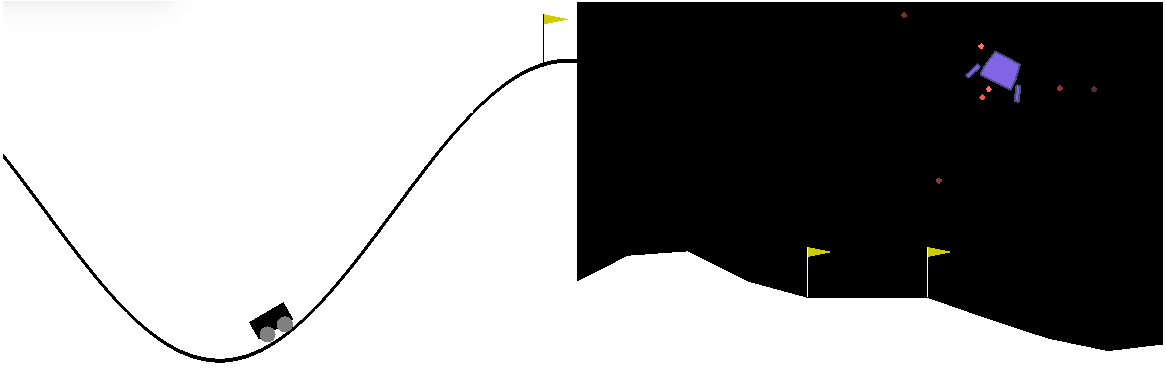
\includegraphics[width = 0.7\columnwidth]{figs/mountainlunar.png}
 \caption{Left: MountainCar Environment, Right: LunarLander Environment.}
\label{fig:mountainlunar}
\end{figure}


%!TEX root = ../authorinstr.tex

\section{Background}

\subsection{Reinforcement Learning}

In Reinforcement Learning problems are modeled as Markov Decision Processes (MDP). An MDP in the context of RL
is a four-valued tuple $(S,A,R,T)$, where $S$ is a set of states that together make up the environment that a RL agent can be in,
 $A$ is a set of actions the agent can take, $R: S \times A \times S \rightarrow \mathbb{R}$, is a reward function mapping a state the agent is in $s_t$,
 an action by the agent $a_t$ and the resulting new state of the agent $s_{t+1}$ to a reward $R(s_t,a_t,s_{t+1})$
 and $T: S \times A \times S \rightarrow [0,1]$ is a series of transition probabilites of $T(s_t,a_t,s_{t+1})$, the probability of the agent
 ending up in a possible state $s_{t+1}$ when it executes action $a_t$ in state $s_t$. \\
 The policy of an agent $\pi: S \times A \rightarrow [0,1]$ is the probability the agent choosing action $a_t$ in state $s_t$. The agent learns by storing values for each
 state or for each combination of possible states and actions, allowing it to optimize its policy by maximizing its expected total discouned reward
 (see equation \ref{eq:opt_pol}, also \cite{zimmer2016neural}).

\begin{equation}
\label{eq:opt_pol}
\pi^* = \operatorname{arg\,max}_{\pi} \mathbb{E}\left [ \sum_{t = 0}^{\infty}\gamma^{t} \times R(s_t,\pi_t(s_t))\right ]
\end{equation}

In equation \eqref{eq:opt_pol} $t$ is a time step and $\gamma$ is the discount factor, which weighs the value of the current reward against the value of potential future rewards.
The discount factor is traditionally defined as being part of a Markov Decision process, but for RL purposes the discount factor is seen as part
of the algorithms and not as part of the MDP, because different algorithms require different discount factors to perform optimally when the model
$(S,A,R,T)$ is kept the same \cite{van2007reinforcement}. In the RL setting of this paper the agent must learn the optimal policy model-free, meaning $R$ and $T$ are not known.
State values or Q-values (values of a certain action in a certain state) are updated, for example on each time step, see the function in equation \ref{eq:upd_q}, where $\alpha$ is the learning rate.

\begin{equation}
\label{eq:upd_q}
Q(s_t,a_t) = Q(s_t,a_t) + \alpha*(r_t + \gamma Q(s_{t+1},a_{t+1}) - Q(s_t, a_t))
\end{equation}

\subsection{Continuous State Space}

When the state space $S$ is continuous, storing the values of states or state action combinations is not possible. However the function $V(s_t)$ that maps states (or $Q(s_t,a_t)$ that maps combinations of states and actions) can be approximated with a Function Approximator. A Multi-Layer Perceptron was used as function approximator and updated the MLP weights using back-propagation.

\subsection{Continuous Action Space}

When the action space $A$ is continuous as well, naively applying the argmax operator for action selection is no longer possible. One solution to this is to use an MLP as a Function Approximator for action selection as well as for determining the value. Another solution is to use a discretized action space as a starting point to find a number of local maxima in the action space, for example by iteratively applying gradient descent on the starting discrete actions, and to finally take the argmax of the local maxima.



%!TEX root = ../authorinstr.tex

\section{Continuous Actor Critic Learning Automaton}
A well established algorithm in Reinforcement Learning (RL) is Continuous Actor Critic Learning Automaton (CACLA)~\cite{van2007reinforcement}. CACLA deals with undiscretized continuous state and action spaces. It implements an Actor Critic system in which both the Actor and Critic are represented by a Multi-Layer Perceptron. In an Actor-Critic system, the Actor is responsible for selecting the current action given the policy and the Critic is used in the calculation of the Temporal Difference (TD)-error which drives the learning of the Actor. The TD learning rule is characterized by equation \eqref{eq:td}, where $\sigma_{t}$ is the TD-difference error as written in \eqref{eq:tderror}. The Actor-Critic system allows for a seperation between the representation of the policy and the value function. A visualization of the Actor-Critic system is shown in Figure~\ref{fig:actorcriticsystem}. In RL problems it is important to be aware of the exploration versus exploitation trade-off; meaning that a decision has to be made between exploration which might lead to an improvement of the current policy or simply the action is selected according to the current policy. An exploration technique that is used often in CACLA is Gaussian Exploration, meaning that an action is calculated around the best action that the current policy provides. To pick a value around the best action, a sample is chosen from a gaussian distribution $N(action, standard deviation)$. The sign of the TD-error ($\sigma_{t} > 0$) is used to determine whether the policy of the Actor has to be updated. To update the Actor in a connectionist way, the performed action $a_{t}$ is used as the target when backpropgating the error using the state $s_{t}$ as input. Since CACLA is an online RL algorithm, the data that is gathered from the interaction of the agent with the environment is used immediately to update the Critic and possibly the Actor. 

\begin{equation}
\label{eq:td}
V(S_{t+1}) = V(S_t) + \alpha_{t} \sigma_{t}
\end{equation}

\begin{equation}
\label{eq:tderror}
\sigma_{t} = r_{t} + \gamma V_{t}(s_{t+1}) - V_{t}(s_{t})
\end{equation}

\begin{figure}[t]
 \centering 
    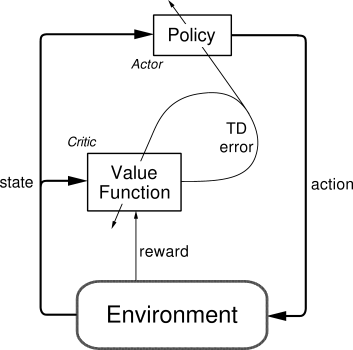
\includegraphics[width = 0.35\columnwidth]{figs/actorcritic.png}
 \caption{Actor Critic system. Reprinted from~\cite{sutton1998reinforcement}}
\label{fig:actorcriticsystem}
\end{figure}





%!TEX root = ../authorinstr.tex

\section{Neural Fitted Actor Critic}
Another RL-method that uses an AC system is Neural Fitted Actor-Critic (NFAC). Where CACLA is an offline AC algorithm, NFAC is an online AC algorithm. This means that a data collection $D_{\pi}$ is built which is filled with experience tuples of the form \{$s_{t}$, $u_{t}$, $a_{t}$, $r_{t+1}$, $s_{t+1}$\}. $s_{t}$ is the state at time $t$, $u_{t}$ is the action the Actor MLP provides, $a_{t}$ is the exploration action which can deviate from $u_{t}$, the reward at time $t+1$ is given by $r_{t+1}$, and finally $s_{t+1}$ is the resulting state after applying $u_{t}$. Every time the agent interacts in the environment, $D_{\pi}$ will be extended with one tuple.

In CACLA, first the Critic is updated and afterwards the Actor. However since the Critic is dependent on the value of the Actor when updating in batches, the Actor is updated first. The Actor is updated towards the exploration action if $\delta > 0$. This is identical for CACLA. NFAC deviates from CACLA by also updating the Actor when $\delta \leq 0$. In that case the update of the Actor is towards the action that the Actor MLP provides. The Critic update is similar to CACLA, but in NFAC the Critic is updated for each experience in $D_{\pi}$. Note that the data collection needs to be emptied after every epoch since the targets used in estimating the new value function are dependent on the current value function. 



%!TEX root = ../authorinstr.tex

\section{Experimental setup}

In this section, the experimental setup used to test the different algorithms will be described. GD-SARSA, CACLA and NFAC are compared in two continuous environments: MountainCar\cite{openaimountaincar} and LunarLander\cite{openailunarlander}. Both environments are OpenAI Gym environments\cite{openaigym}, which is a toolkit for comparing reinforcement learning algorithms.  Agent performance is measured by looking at the average reward over the best 100 epochs. The reward function is given by the OpenAI environment and shown in more detail in their respective subsections. Each simulation run consisted of 2000 epochs, each of which had a maximum of 10000 time steps. Learning rates, discount factors and numbers of hidden nodes for the MountainCar and LunarLander environments can be found in table \ref{tab:mntparam} and table \ref{tab:lunarparam} respectively. 

\begin{table}
\centering
\label{tab:mntparam}
\begin{tabular}{r|llll}
                     & learning rate & discount factor & number of hidden nodes \\\hline
SARSA & N          & P               & M         \\
CACLA & A          & B               & actor: F, critic: G         \\
NFAC    & X          & Y              & actor: H, critic: I        
\end{tabular}
\caption{MountainCar network parameters per algorithm}
\end{table}

\begin{table}
\centering
\label{tab:lunarparam}
\begin{tabular}{r|llll}
                     & learning rate & discount factor & number of hidden nodes \\\hline
SARSA & N          & P               & M         \\
CACLA & A          & B               & actor: F, critic: G         \\
NFAC    & X          & Y              & actor: H, critic: I        
\end{tabular}
\caption{LunarLander network parameters per algorithm}
\end{table}



GD-SARSA used $\epsilon$-greedy exploration, which was first set to 1.0, resulting initially in a fully pseudo-random behaviour. This exploration rate decayed over epochs, and is equal to $0.99^{N-1}$, where N is the current epoch. Since the experiments run for 2000 epochs, this means that the final exploration rate is $1.86*10^{-9}$.   

NFAC and CACLA both used gaussian exploration.  A random value sampled from a gaussian distribution($\mu=0$ $\sigma=1$) was multiplied by a value $\Sigma=10$. This value was added to the output of the MLP and finally clamped to be in the range [$-1$,$1$]. This $\Sigma$ decayed over epochs and is equal to  $10 * 0.99^{N-1}$, where N is the current epoch. Since the experiments run for 2000 epochs, this means that the final exploration rate is $1.86*10^{-8}$. Since initially the exploration rate is very high, this ensures that the agent will quickly reach its goal. [[The exploration rate is diminshed over time since then it can rely more on its learned behavior rather than the noise added by the gaussion value.]] 




%!TEX root = ../authorinstr.tex

\section{Conclusions and further work}
Two different environments are used to compare the performance of the three different RL algorithms. ... performed best in the MountainCar environment obtaining ... Results indicate that ... performs best in the LunarLander environment providing a ... To conclude, SARSA/CACLA/NFAC provides the best results using the parameters ... in MountainCar whereas SARSA/CACLA/NFAC with ... gives the best results for LunarLander. This AGREES/DISAGREES with previous expectations that were stated earlier. However one should note that more data needs to be collected to be more certain about the validity of the results, but due to time restrictions a limited amount of trials are rendered in this research.  

Further work needs to be done in testing different input representations. The OpenAI environments provide an initial state and a new state after every action performed. One can alter the state representation before it is used by the function approximator. An attempted input representation was representing each state value by N units. Each unit is responsible for a range of values; e.g. the range [-1, 1] can be represented in steps of 0.1 by choosing $N=20$ units. Then the value -0.85 is represented by the second hidden unit, so this value is set to 1. The two neighbouring states are set to 0.5 to keep the input representation continuous. This is done for each state value and the result is a concatenated vector holding the new state. Another attempted approach is similar as before, but instead of setting the neighbouring states to 0.5, a convolution is performed with a gaussian window. This way the input can approximate a gaussian even better. Results obtained with these approaches were not evidently better on a first glance. However this should be extensively investigated in further research. Additionally more research should be done with other environments, to be able to generalize more about the performance of Neural Fitted Actor-Critic.



%!TEX root = ../authorinstr.tex

\section{Contributions}



\bibliographystyle{plain}
\bibliography{mybibfile.bib}



\end{document}







